\documentclass[11pt,letterpaper]{article}

% packetages pour écrire en français
\usepackage[french]{babel}
\usepackage[utf8]{inputenc}
\usepackage[T1]{fontenc}

% pour les maths, les graphiques et la navigation dans le pdf
\usepackage{amsmath, amssymb, mathtools, mathrsfs, bm, array, units, amsthm, dsfont}
\usepackage{graphicx,caption}
\usepackage{hyperref}
\usepackage{subcaption}
\usepackage{physics} %très utile pour écrire plus rapidement des matrices, des dérivées, etc. Allez voir la documentation!

% marges, police de caractère et header
\usepackage{geometry}
\geometry{top=30mm, bottom=30mm, left=20mm, right=20mm}
\usepackage{cochineal}
\usepackage{fancyhdr}
\pagestyle{fancy}
\usepackage{float}
\usepackage{pdfpages}
\parindent=0mm % pas d'indentation
\setlength\headheight{13.6pt}


% nouvelles commandes pour écrire des équations plus vite avec leur label
\newcommand{\beq}[1]{\begin{equation} \label{#1}}
\def\enq{\end{equation}}

\begin{document}  	
\thispagestyle{empty} % pas de header sur la première page
\begin{center}

{\large LRIO}
\hfill
{\large {Philippe Truchon}}\\


\hfill
{\large \textsc{}} \\~\\
{\Large \textbf{Calcul d'aberrations avec PSM (Point Source Microscope}}\\~\\
{\large {mai 2022}}
\end{center}
\section{Liste de matériel}
\begin{itemize}
    \item Source ponctuel laser collimaté (diode laser avec fibre optique monomode utilisée)
    \item Lentilles avec montures rotatives
    \item 3 bases en translation et une base en rotation
    \item Le PSM (incluant l'ordinateur)
\end{itemize}
\section{Montage}
\begin{figure}[H]
    \centering
    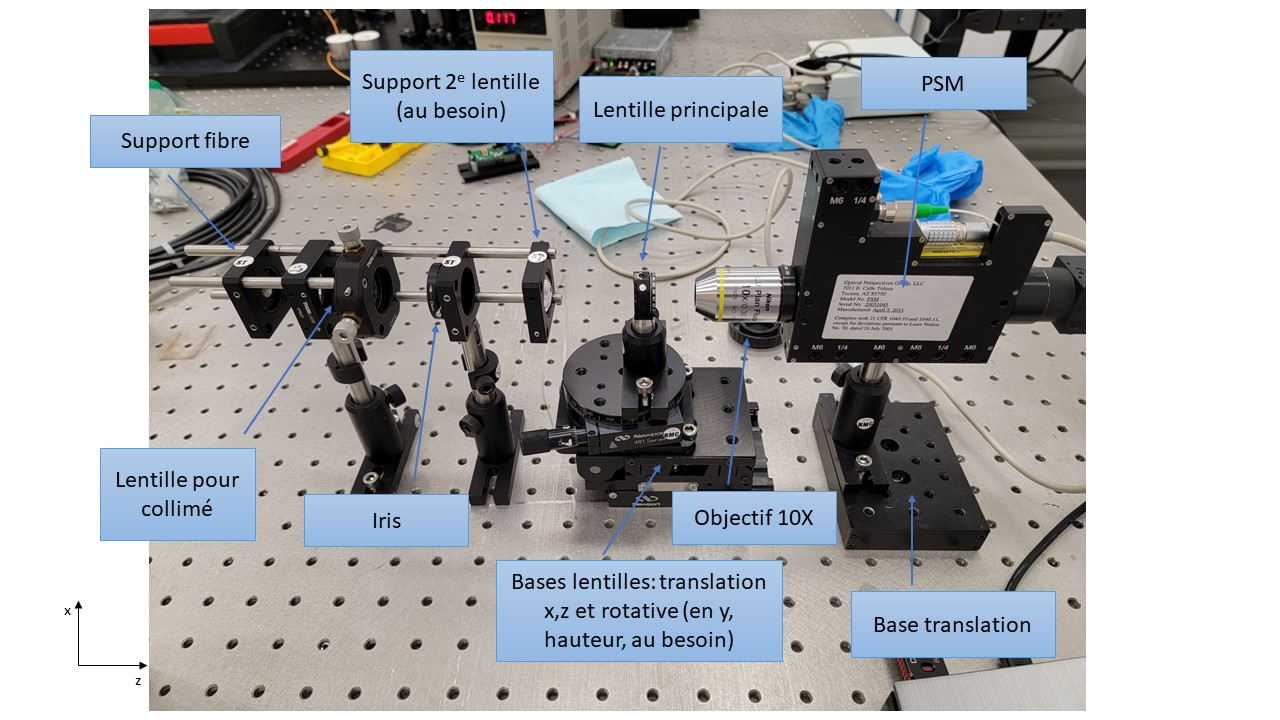
\includegraphics[scale=0.5]{montage_psm.jpg}
    \caption{Montage utilisé pour l'expérience de caractérisation des aberrations à l'aide du PSM.}
    \label{montage}
\end{figure}
Une source fibrée monomode doit être connectée au support à fibre pour réaliser l'expérience. Le détail des lentilles sera exploré avec les résultats.
\section{Protocole}
\begin{enumerate}
    \item Allumé la source laser pour l'alignement (intensité faible, mais visible)
    \item Aligné la source laser pour qu'elle soit capté par le PSM. Se servir de la source du PSM au besoin pour vérifier que la faisceau soit bien centré dans les composants optiques
    \item Trouver le point de focus en déplaçant la lentille principale en z (monture translation)
    \item Prendre une photo avec le PSM au point de meilleur focus visuel et la nommer '0.png'
    \item Déplacer la lentille principale sur l'axe z avec la base en translation à intervalles égaux de chaque côtés du point 0 et prendre des images à tous ces points
    \item Exporter ces images regroupés dans un dossier
\end{enumerate}
\section{Traitement des images}
Le traitement des images se fait avec le code python suivant \url{Lien_github_à_venir}. Le code est de type Jupyter Notebook, donc il peut être nécessaire d'installer l'extension sur VsCode. Il faut aussi avoir installer numpy, matplolib et openCV.
\section{Exemple de résultat}
Ces résultats sont obtenus avec un montage ne contenant pas la deuxième lentille et la lentille principale à un diamètre de 1" est une focale de 15 mm. L'iris était ouvert à 8 mm\footnote{Les images peuvent être vues avec le lien GitHub du code python}.
\begin{figure}[H]
    \centering
    \includegraphics[scale=0.3]{test23_psm.jpg}
    \caption{Allure de la source ponctuel et des ses aberrations pour un bon alignement.}
    \label{test23}
\end{figure}
\begin{figure}[H]
    \centering
\subfloat[]{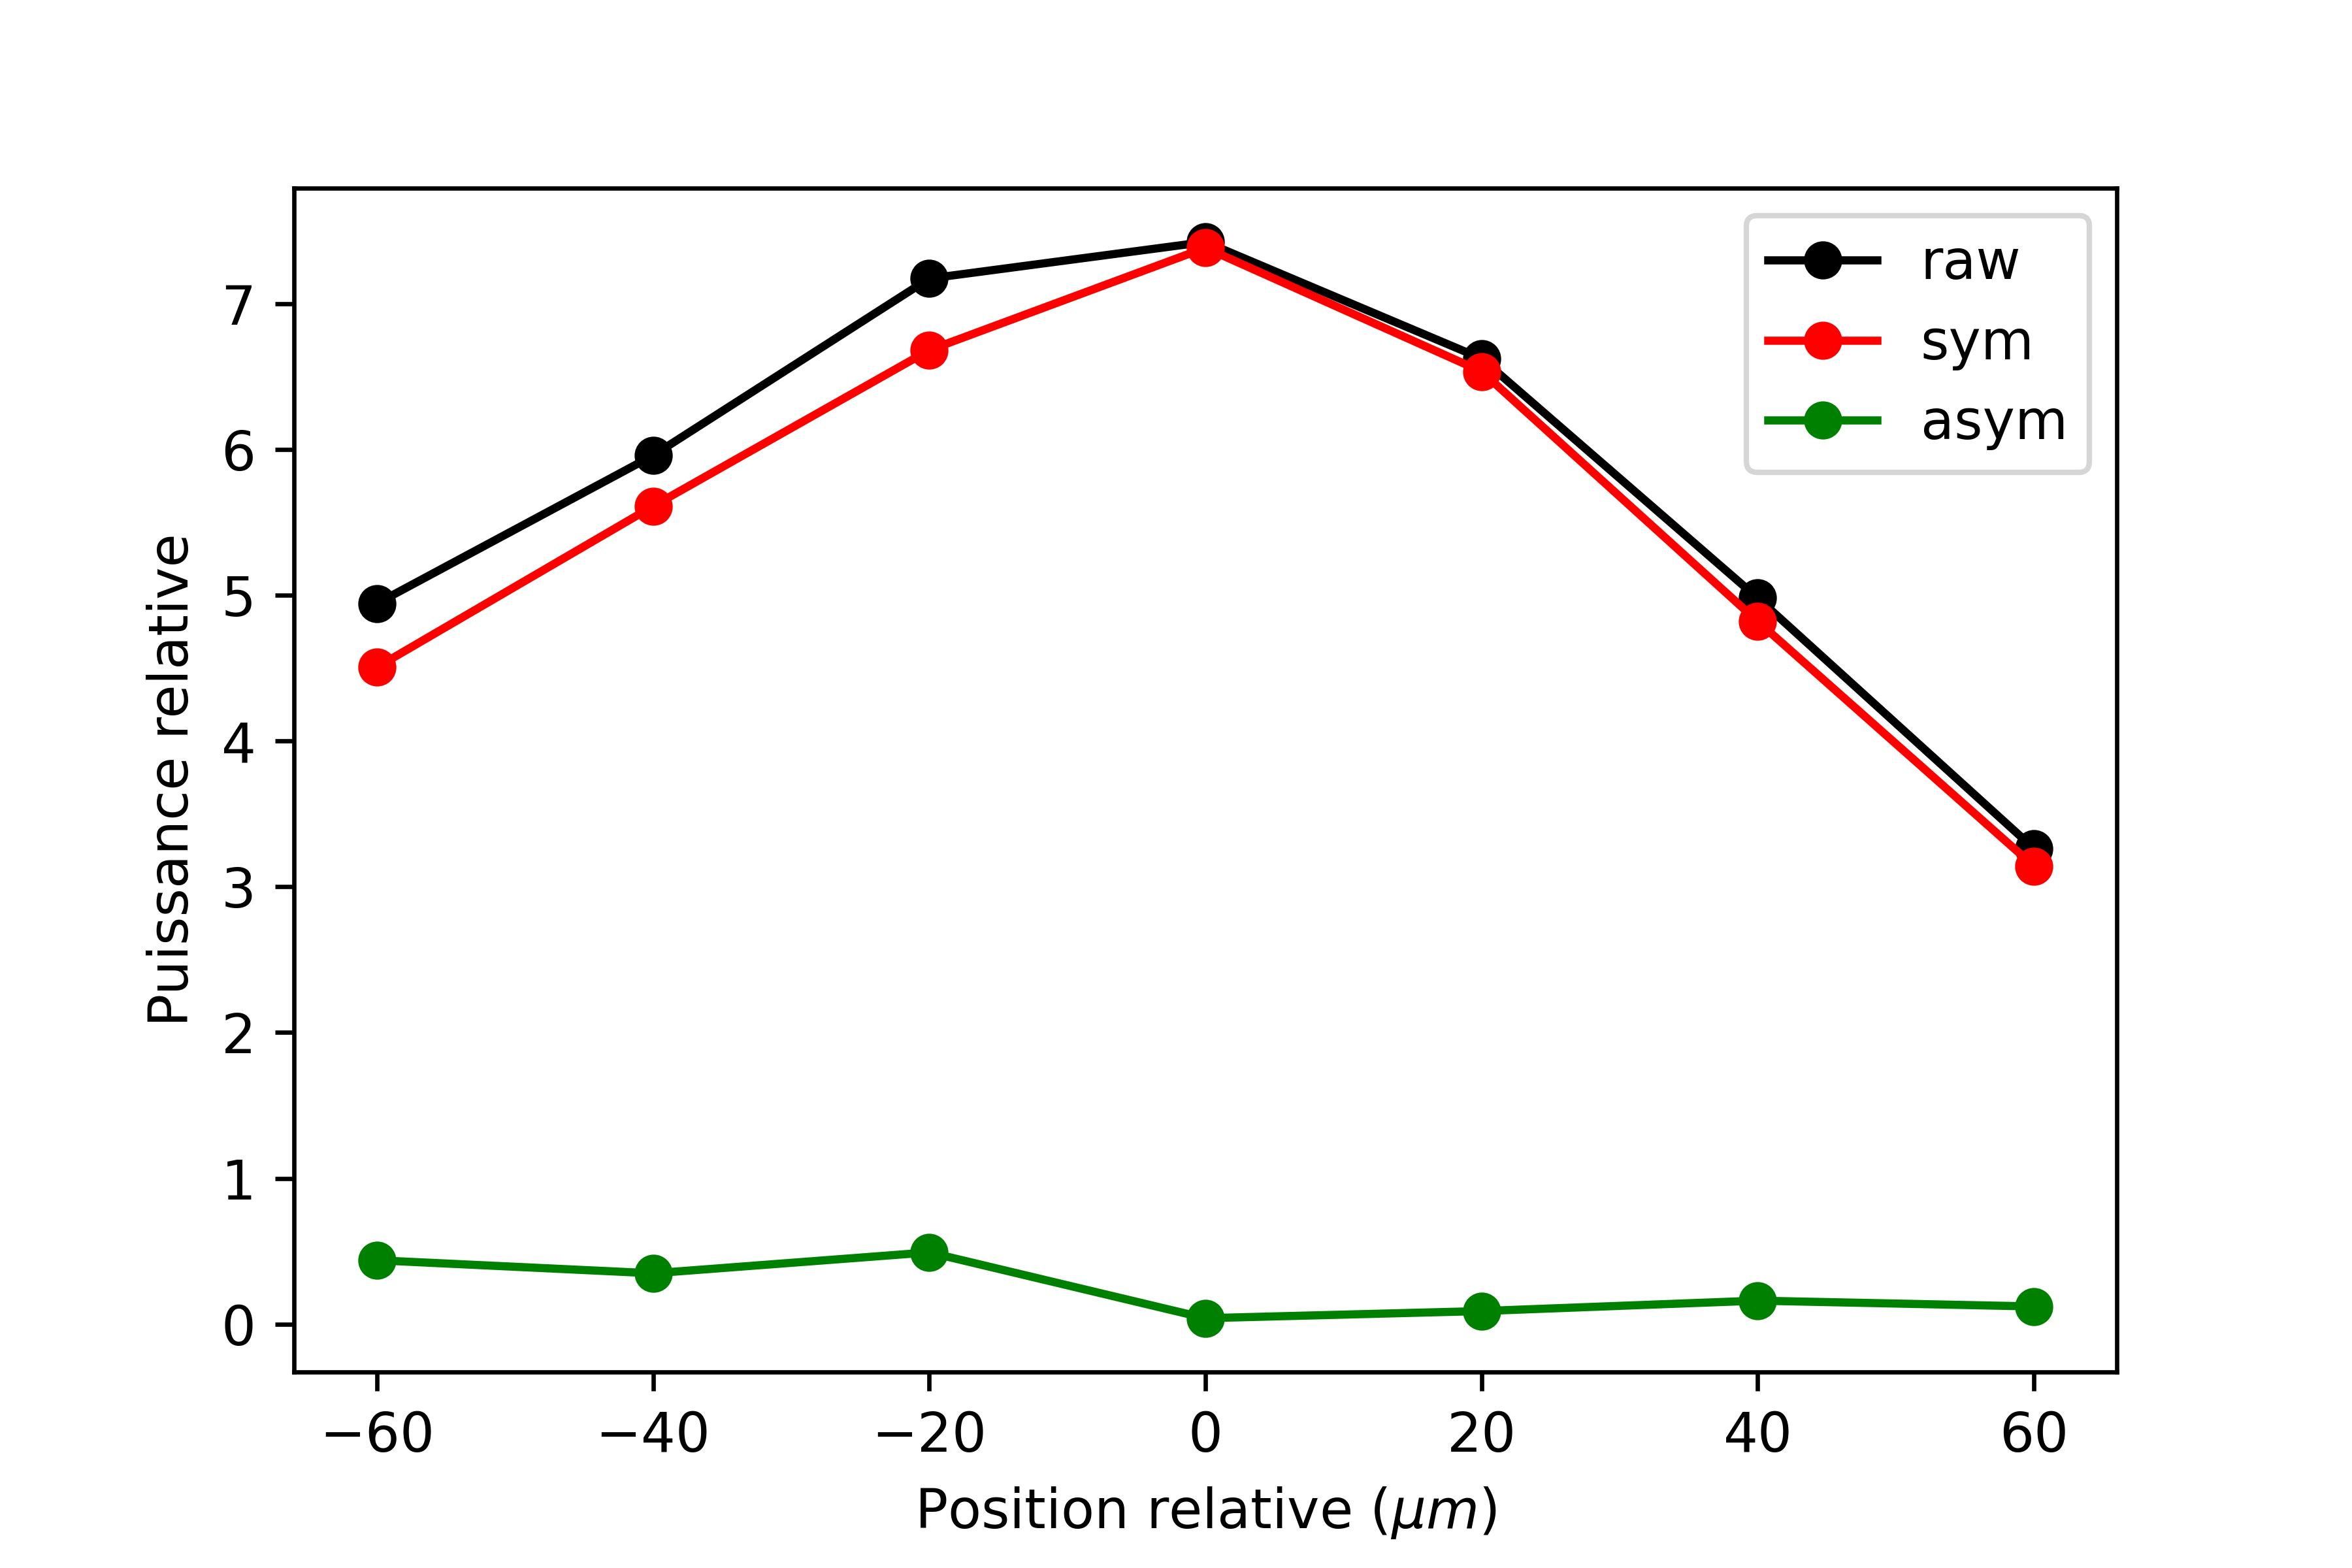
\includegraphics[scale=0.6, angle=0]{test23_psm_power1.jpg}}
\subfloat[]{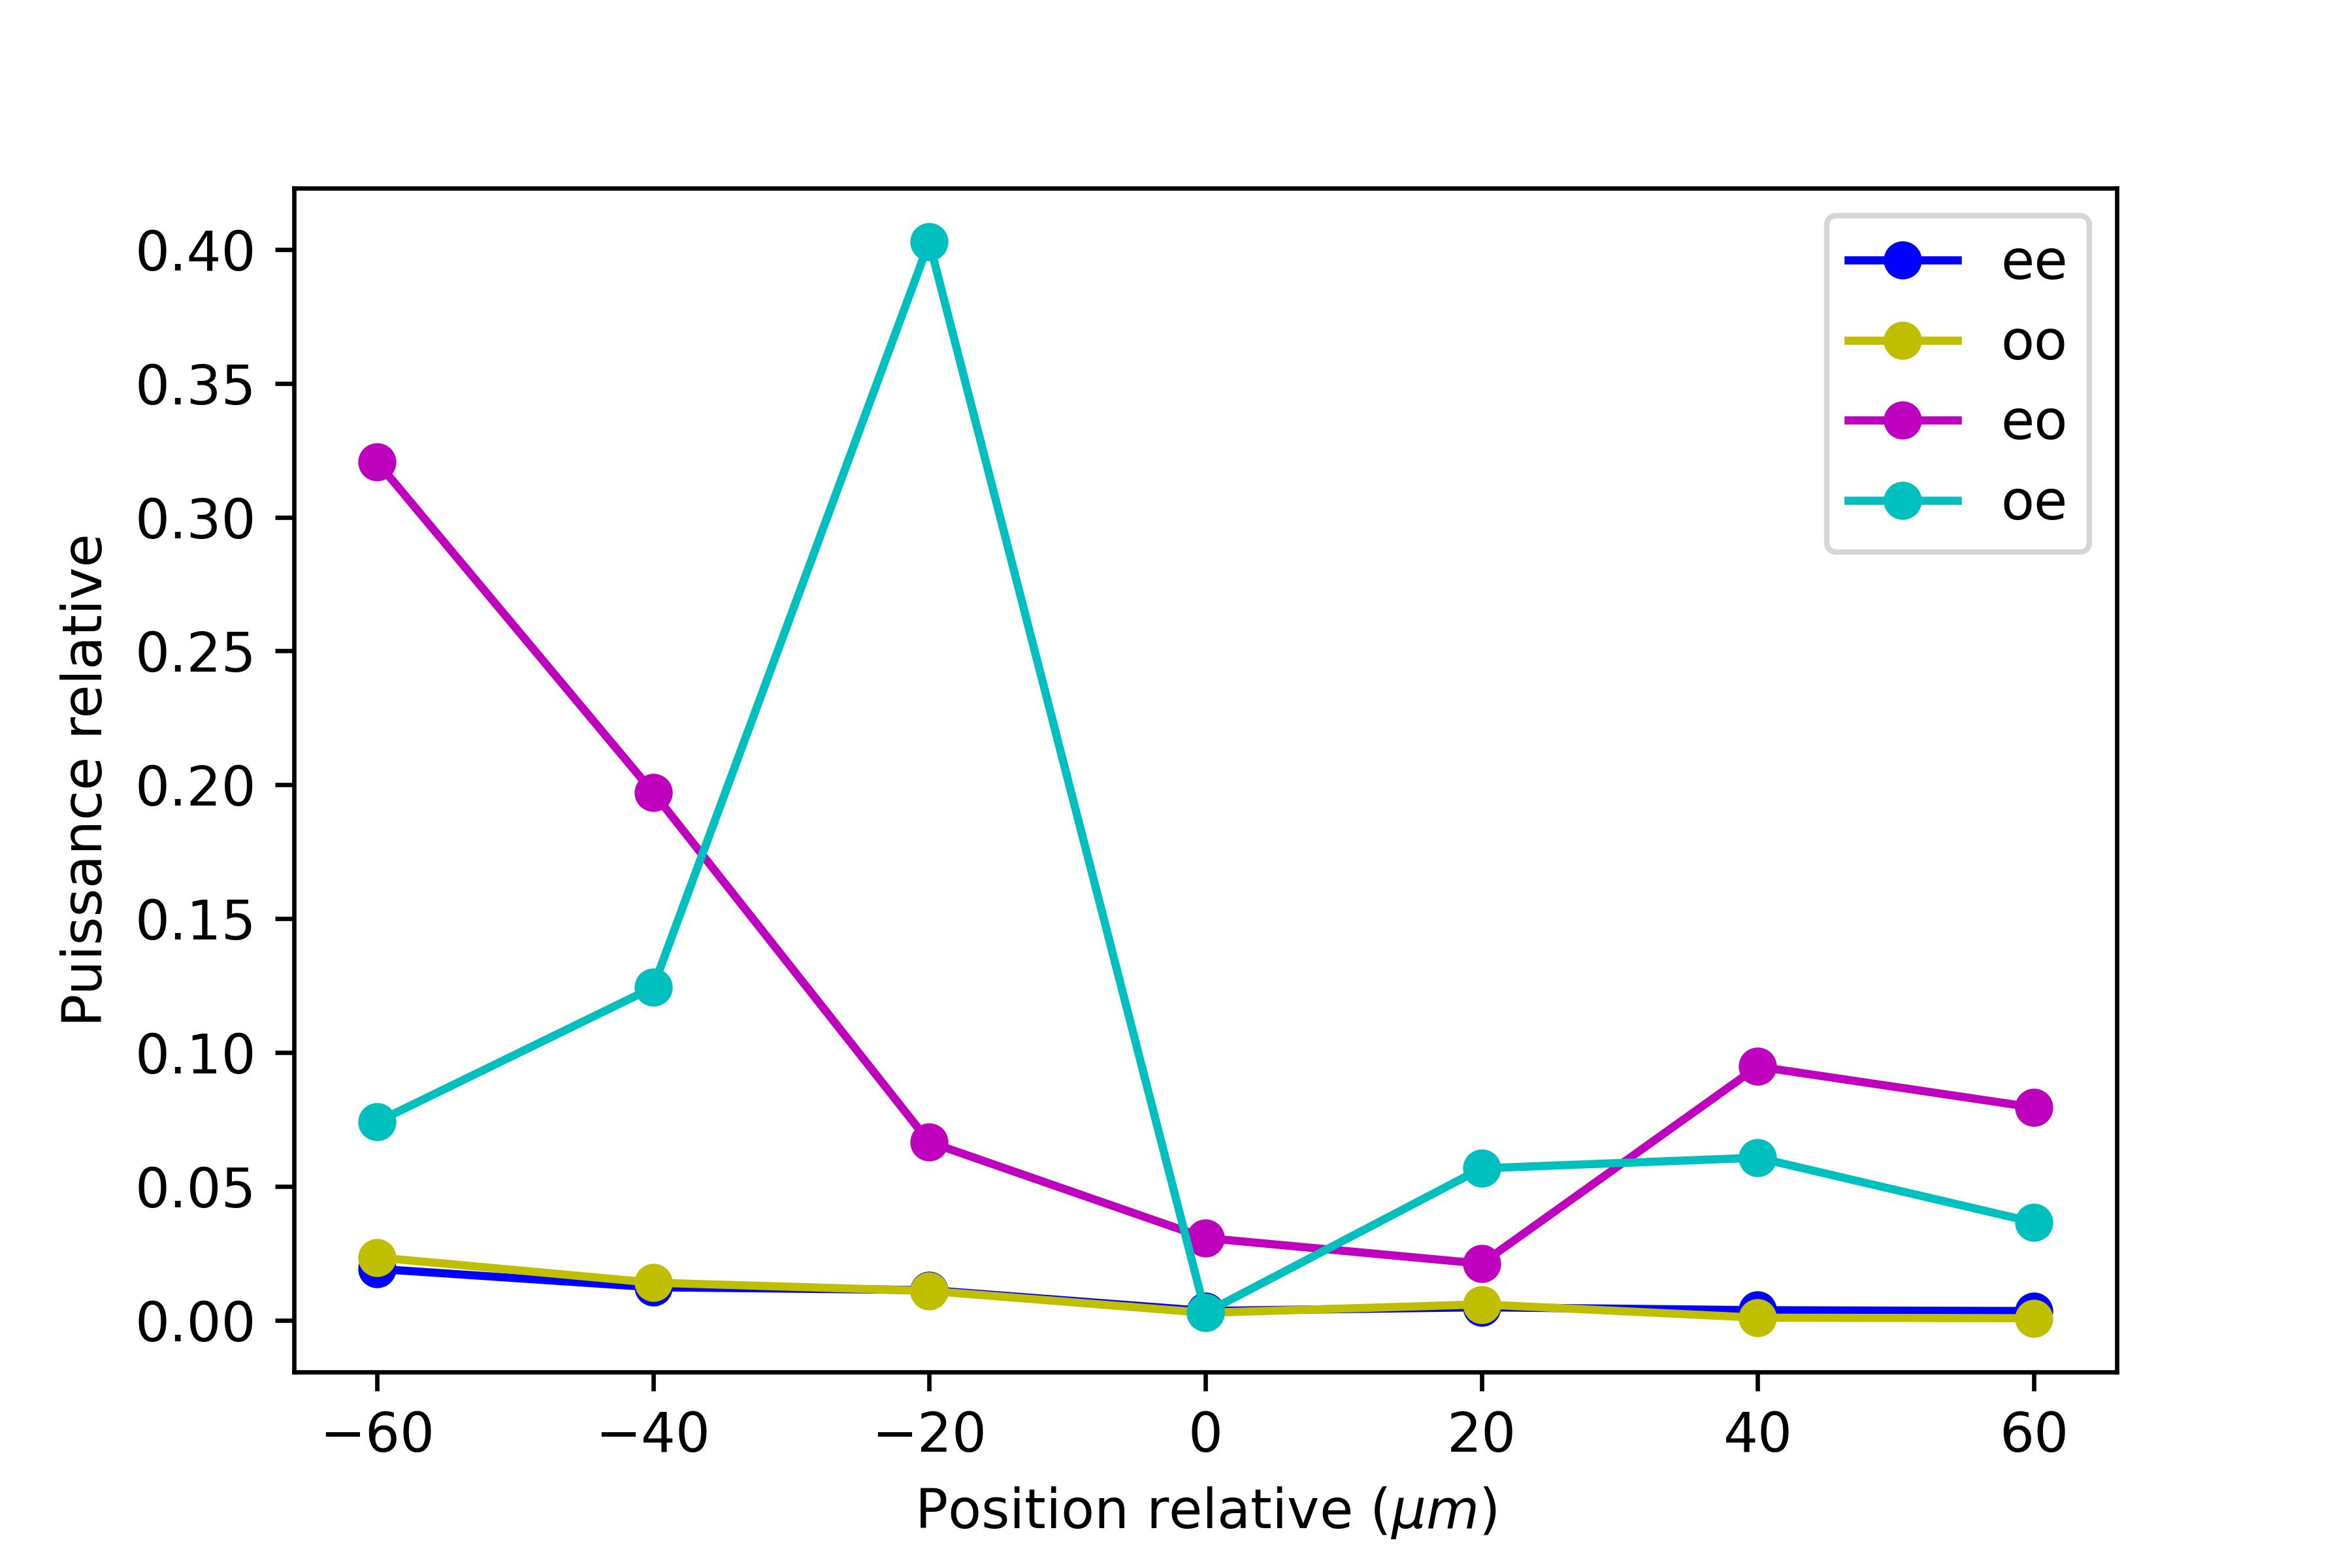
\includegraphics[scale=0.6, angle=0]{test23_psm_power2.jpg}}

\caption{Puissance relative des différentes images de la figure \ref{test23}.}
\label{fig4}
\end{figure}
Avec 'raw' représentant la photo originale rognée, 'sym' la partie symétrique de 'raw' et asym la différence de 'raw' et 'sym'. De plus, ee représente l'astigmatisme à 0\textsuperscript{o}, oo l'astigmatisme à 45\textsuperscript{o}, eo le coma en y et oe le coma en x. On observe des pics inattendus pour les composantes eo et oe. Ceci peut être causé, surtout avec peu d'aberrations, par un vrai centre entre 2 pixels de l'image créant des fausses aberrations en x et y.
\begin{figure}[H]
    \centering
    \includegraphics[scale=0.3]{test26_psm.jpg}
    \caption{Allure de la source ponctuel et des ses aberrations pour un angle de lentille de 10\textsuperscript{o}}
    \label{test27}
\end{figure}
\begin{figure}[H]
    \centering
\subfloat[]{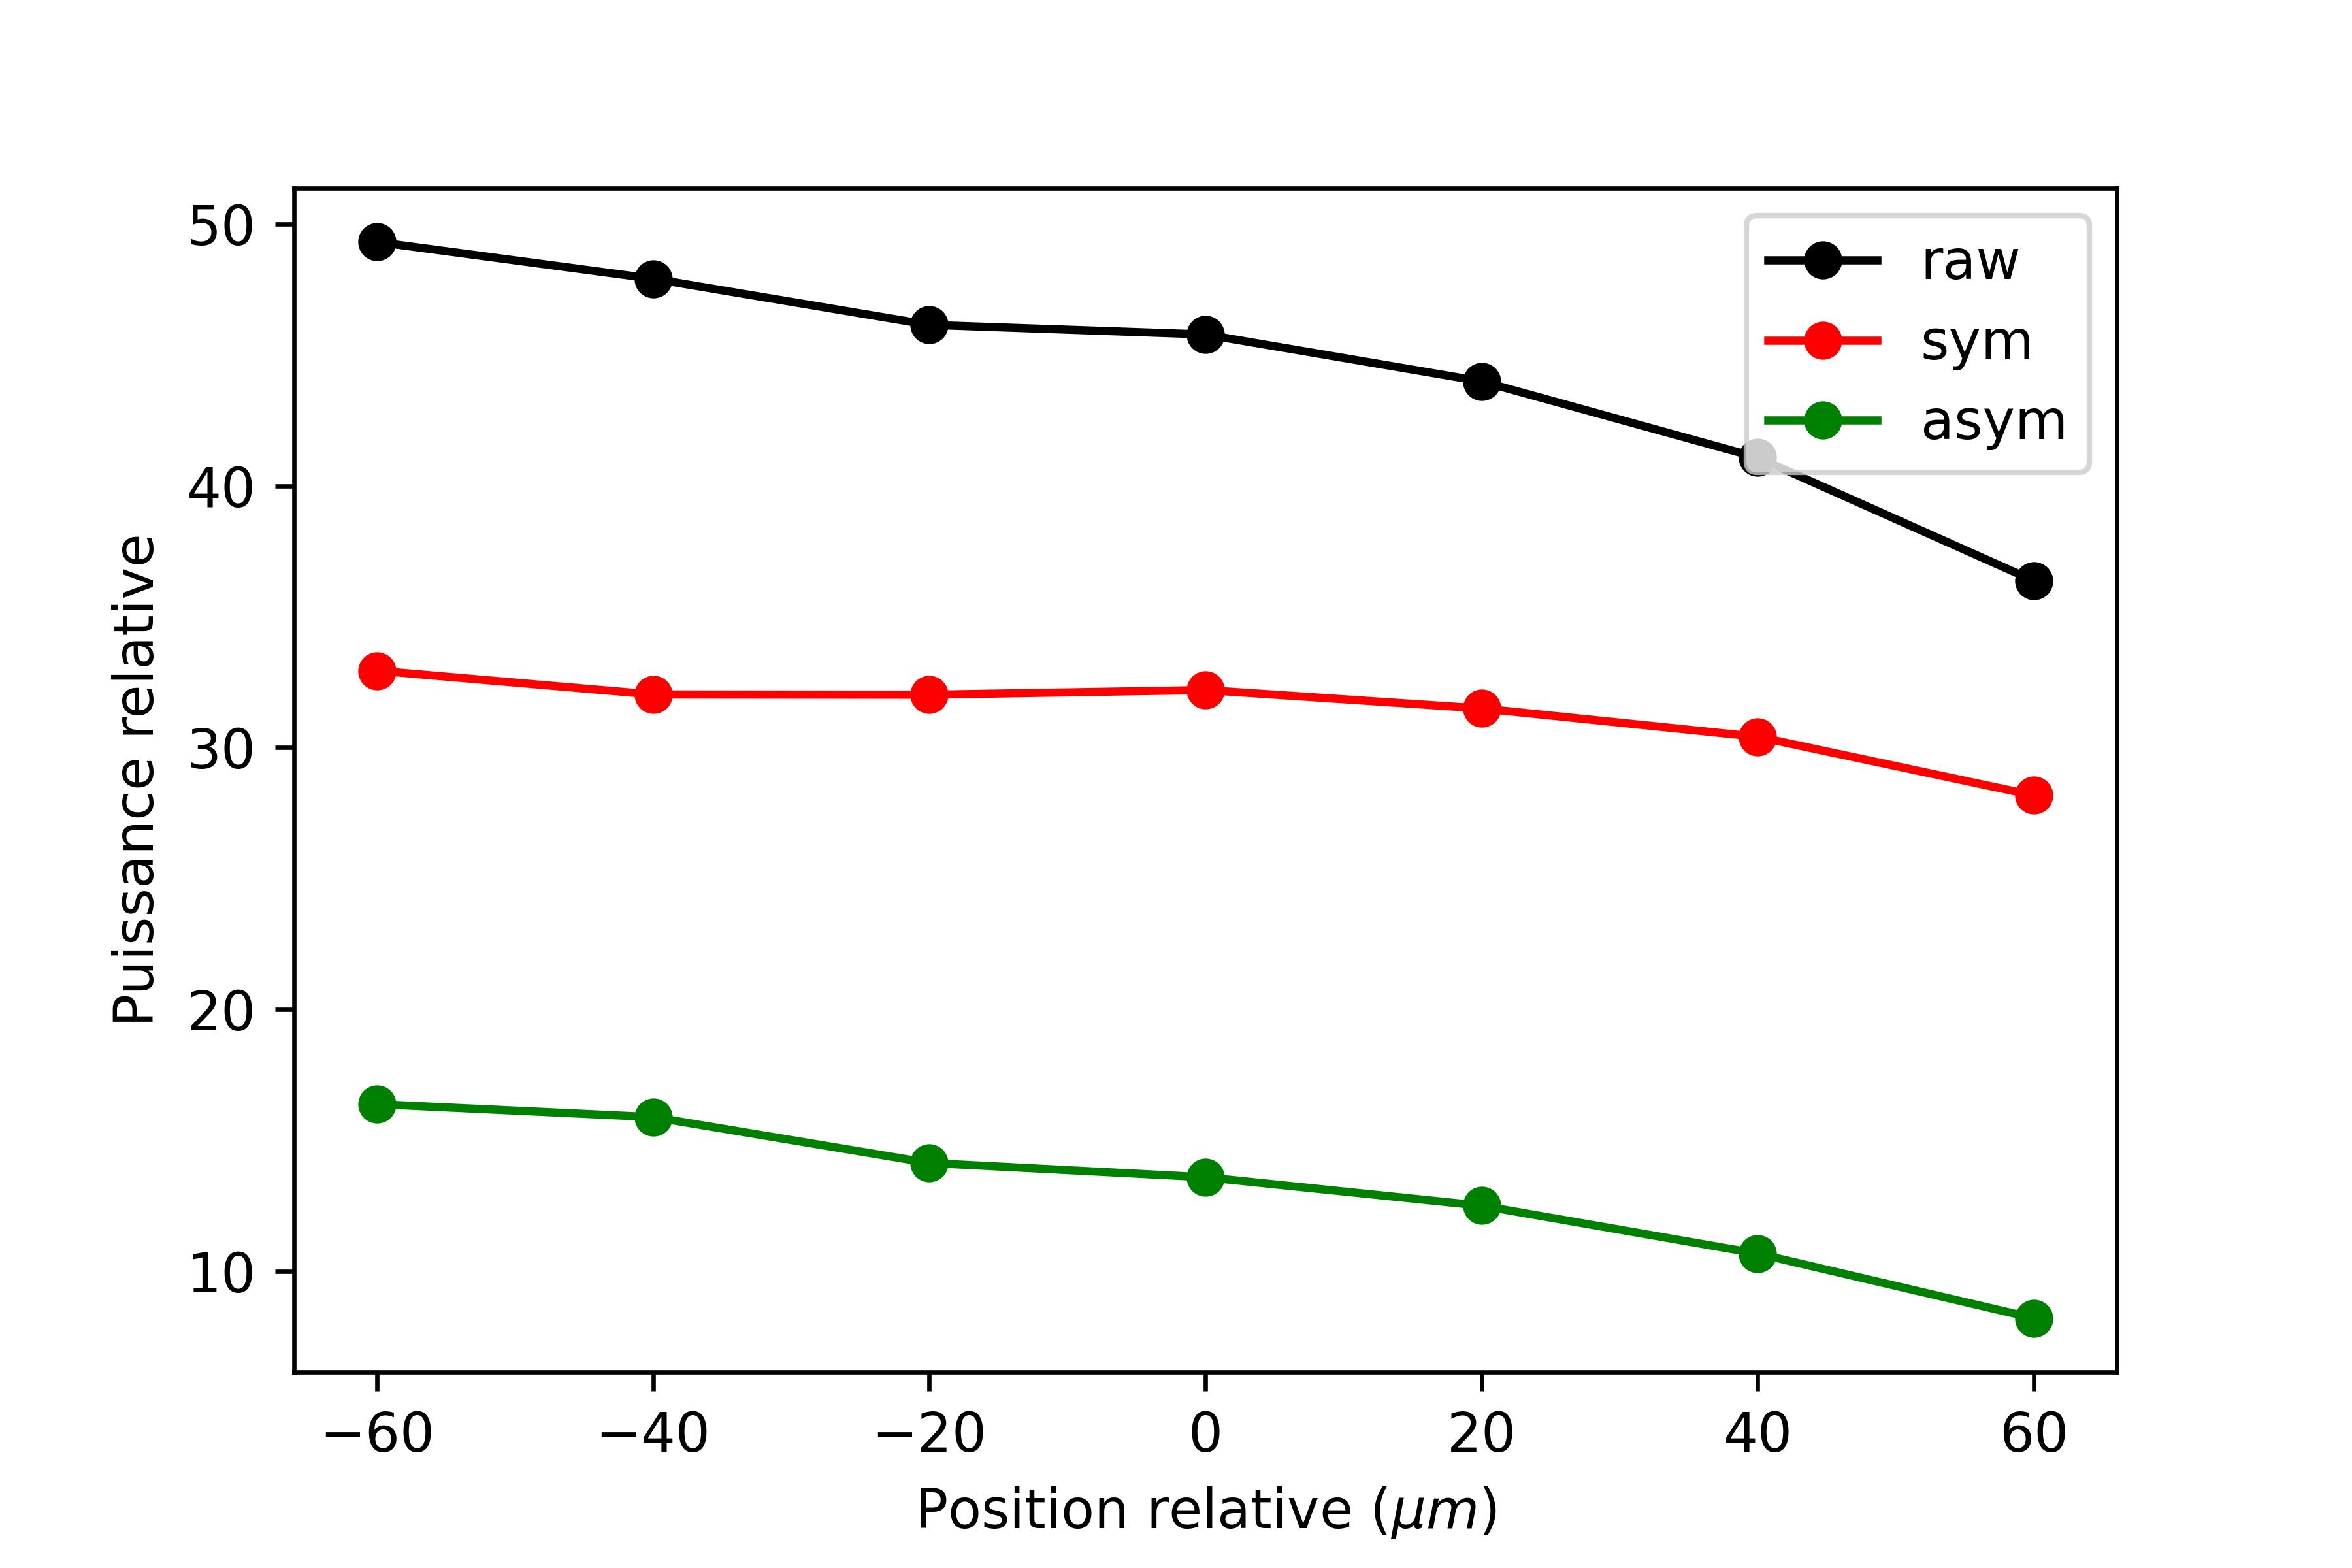
\includegraphics[scale=0.6, angle=0]{test26_psm_power1.jpg}}
\subfloat[]{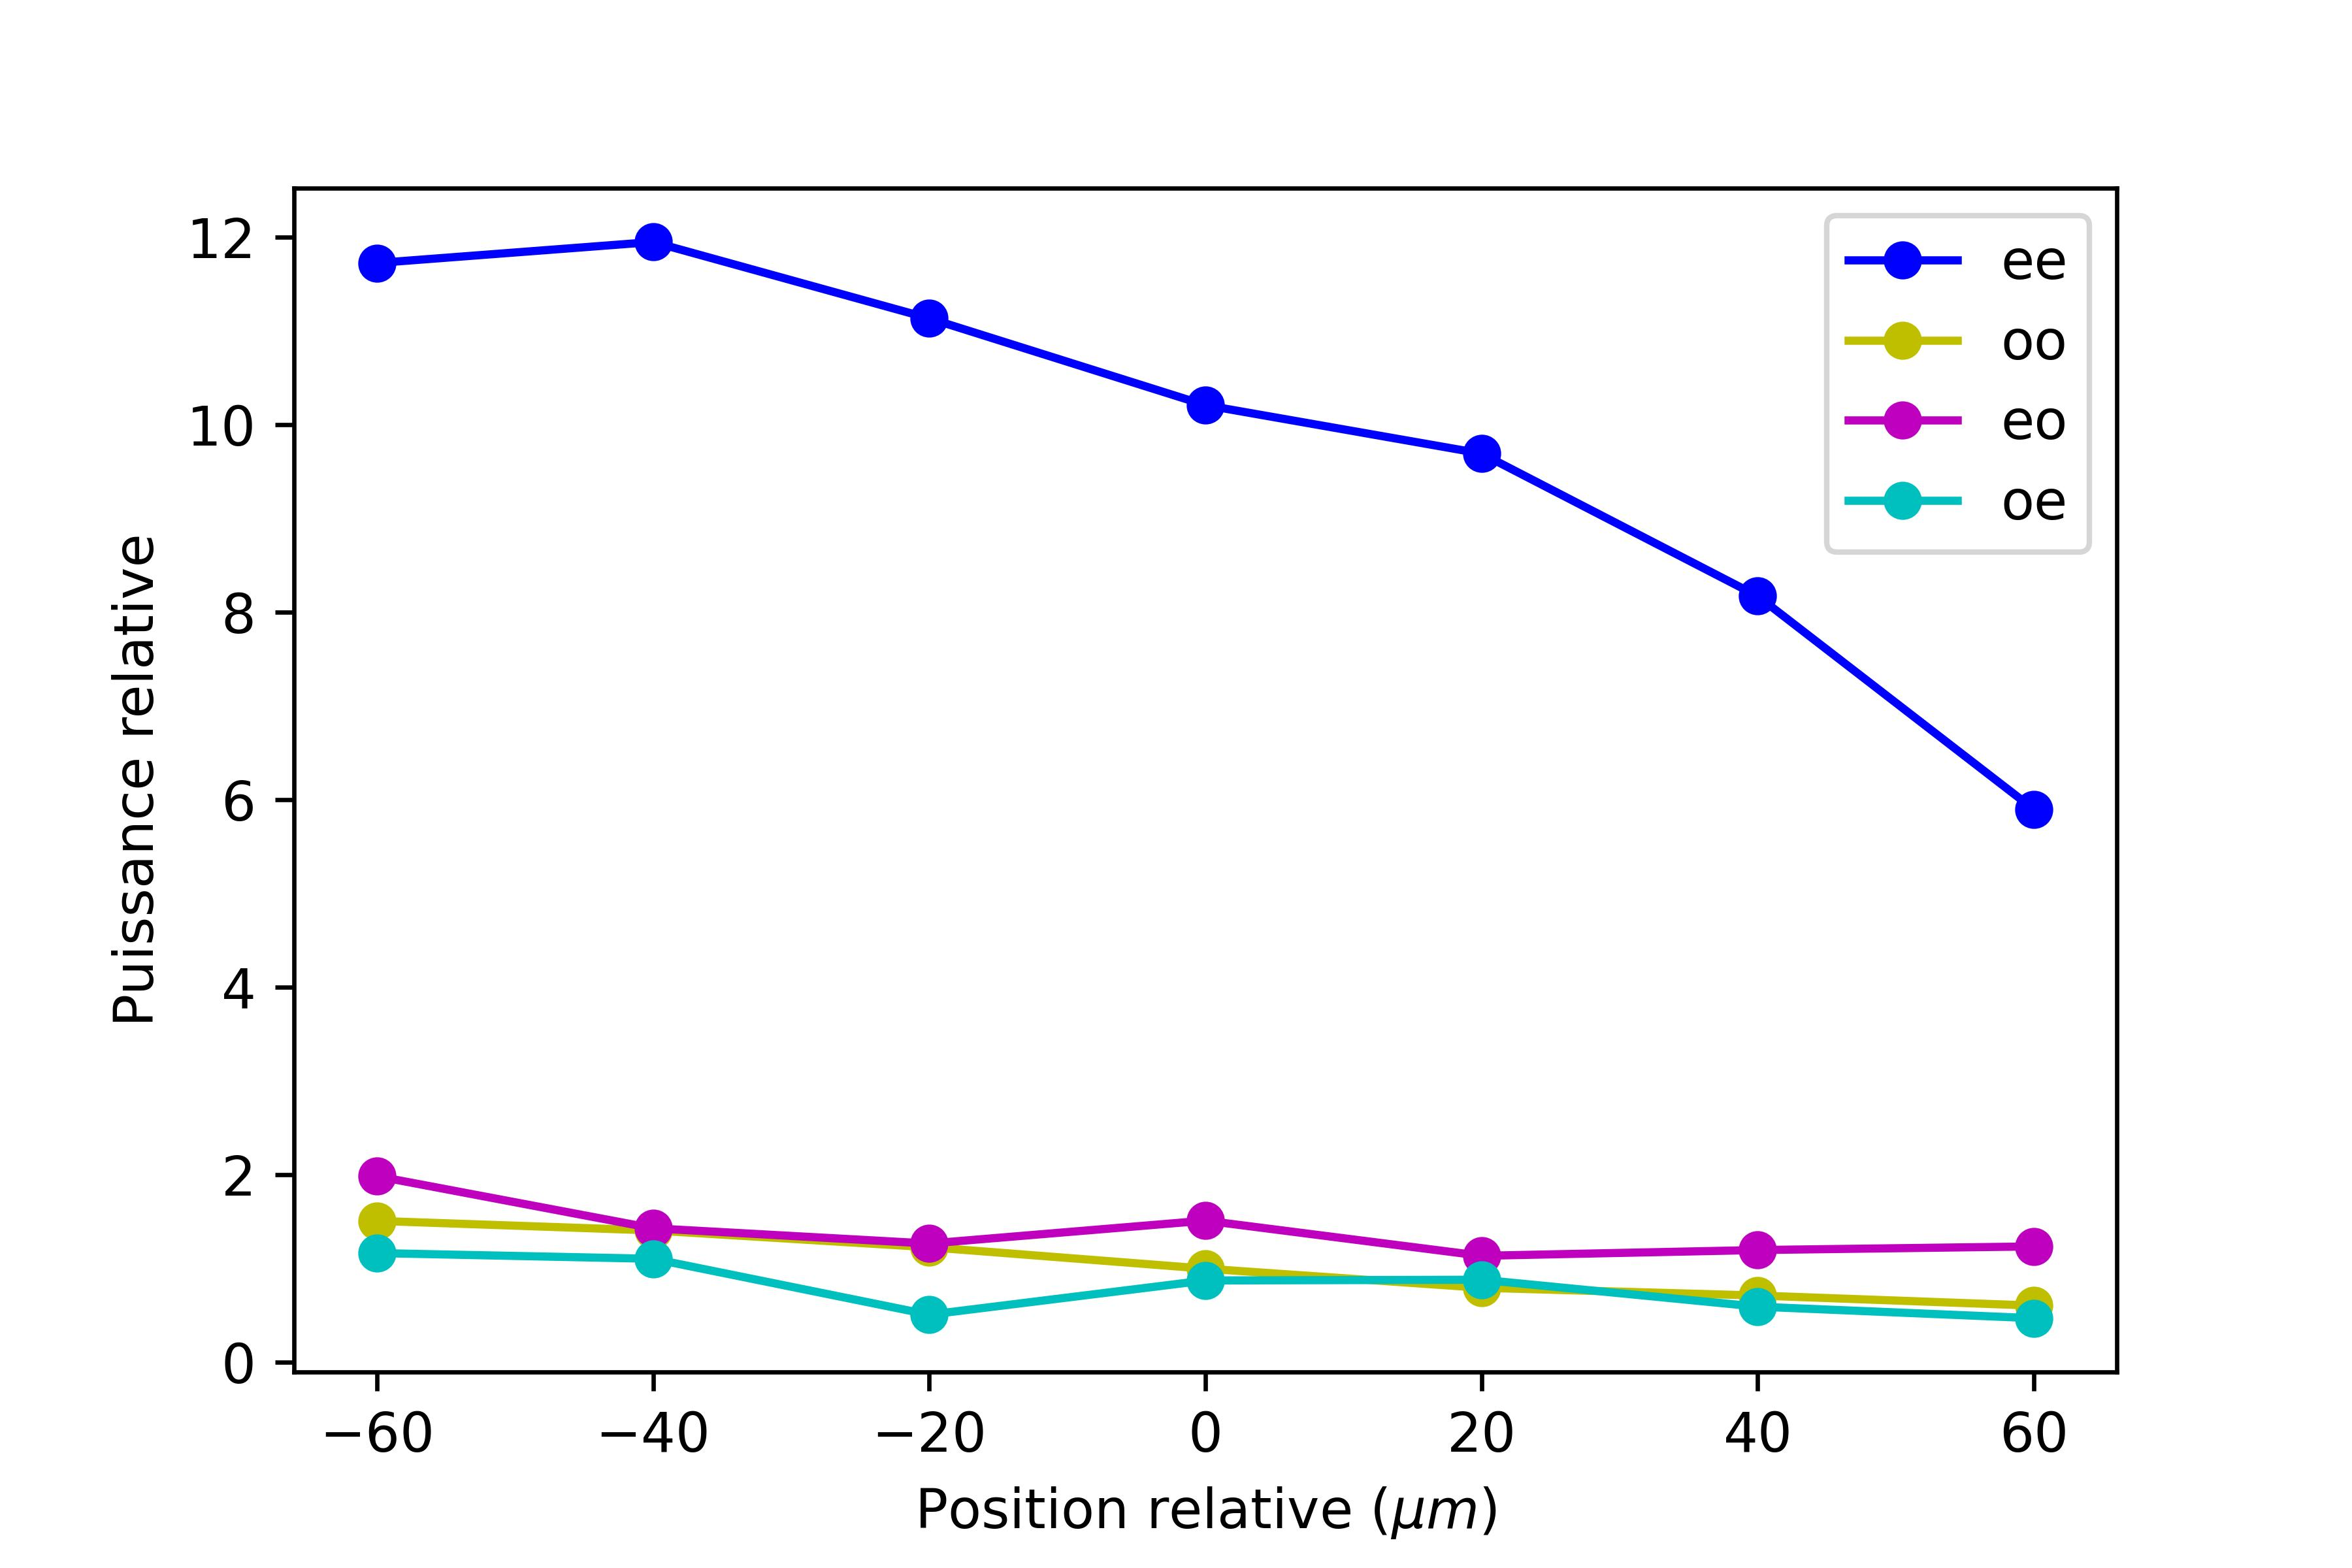
\includegraphics[scale=0.6, angle=0]{test26_psm_power2.jpg}}

\caption{Puissance relative des différentes images de la figure \ref{test27}.}
\label{fig4}
\end{figure}
Dans ce cas, on observe que l'angle de  la lentille a causé une augmentation des aberrations, principalement l'astigmatisme à 0\textsuperscript{o}. On observe aussi une PSF dans ce cas, mais elle est considéré symétrique sans aberrations, donc elle suit aussi à même titre qu'un point les aberrations de lentilles et elle peut être ignorer dans l'analyse
\end{document}
